\subsection{bpmmode Struct Reference}
\label{structbpmmode}\index{bpmmode@{bpmmode}}
{\tt \#include $<$bpm\_\-interface.h$>$}

Collaboration diagram for bpmmode:\nopagebreak
\begin{figure}[H]
\begin{center}
\leavevmode
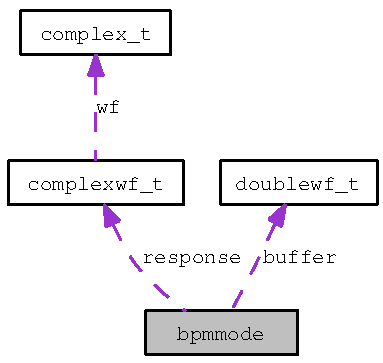
\includegraphics[width=110pt]{structbpmmode__coll__graph}
\end{center}
\end{figure}


\subsubsection{Detailed Description}
This structure defines a BPM resonant mode which is defined by it's resonant frequency, Q factor and sensitivities to the beam charge, slope and bunch tilt. 

Definition at line 282 of file bpm\_\-interface.h.\subsubsection*{Data Fields}
\begin{CompactItemize}
\item 
char {\bf name} [20]
\item 
double {\bf frequency}
\item 
double {\bf Q}
\item 
int {\bf order}
\item 
enum {\bf bpmpol\_\-t} {\bf polarisation}
\item 
double {\bf sensitivity}
\item 
{\bf complexwf\_\-t} $\ast$ {\bf response}
\item 
{\bf doublewf\_\-t} $\ast$ {\bf buffer}
\end{CompactItemize}


\subsubsection{Field Documentation}
\index{bpmmode@{bpmmode}!name@{name}}
\index{name@{name}!bpmmode@{bpmmode}}
\paragraph[name]{\setlength{\rightskip}{0pt plus 5cm}char {\bf bpmmode::name}[20]}\hfill\label{structbpmmode_8f3ec37ef0fdda0eeec8bf9a056f175a}


The name for the BPM mode, e.g \char`\"{}dipolex\char`\"{} 

Definition at line 283 of file bpm\_\-interface.h.

Referenced by generate\_\-bpmsignal().\index{bpmmode@{bpmmode}!frequency@{frequency}}
\index{frequency@{frequency}!bpmmode@{bpmmode}}
\paragraph[frequency]{\setlength{\rightskip}{0pt plus 5cm}double {\bf bpmmode::frequency}}\hfill\label{structbpmmode_b17dc935c70d7e9aec15d6ce93b14046}


The resonant frequency of the mode 

Definition at line 284 of file bpm\_\-interface.h.

Referenced by get\_\-mode\_\-amplitude(), and get\_\-mode\_\-response().\index{bpmmode@{bpmmode}!Q@{Q}}
\index{Q@{Q}!bpmmode@{bpmmode}}
\paragraph[Q]{\setlength{\rightskip}{0pt plus 5cm}double {\bf bpmmode::Q}}\hfill\label{structbpmmode_0d153f15610441366c0e2eb09089f092}


The Q factor for the mode 

Definition at line 285 of file bpm\_\-interface.h.

Referenced by get\_\-mode\_\-response().\index{bpmmode@{bpmmode}!order@{order}}
\index{order@{order}!bpmmode@{bpmmode}}
\paragraph[order]{\setlength{\rightskip}{0pt plus 5cm}int {\bf bpmmode::order}}\hfill\label{structbpmmode_90ab04d3b70f66e6a65e2399d92f018a}


The mode order, 0:monopole, 1:dipole, 2:quadrupole... 

Definition at line 286 of file bpm\_\-interface.h.

Referenced by add\_\-mode\_\-response(), get\_\-mode\_\-amplitude(), and get\_\-mode\_\-response().\index{bpmmode@{bpmmode}!polarisation@{polarisation}}
\index{polarisation@{polarisation}!bpmmode@{bpmmode}}
\paragraph[polarisation]{\setlength{\rightskip}{0pt plus 5cm}enum {\bf bpmpol\_\-t} {\bf bpmmode::polarisation}}\hfill\label{structbpmmode_72e607b92a918c1294d30523b39cff5b}


The mode polarisation: horiz, vert 

Definition at line 287 of file bpm\_\-interface.h.

Referenced by get\_\-mode\_\-amplitude().\index{bpmmode@{bpmmode}!sensitivity@{sensitivity}}
\index{sensitivity@{sensitivity}!bpmmode@{bpmmode}}
\paragraph[sensitivity]{\setlength{\rightskip}{0pt plus 5cm}double {\bf bpmmode::sensitivity}}\hfill\label{structbpmmode_9e0125d3567d1be32ce516fddf432e04}


The sensitivity of the mode, units depend on order 

Definition at line 288 of file bpm\_\-interface.h.

Referenced by get\_\-mode\_\-amplitude().\index{bpmmode@{bpmmode}!response@{response}}
\index{response@{response}!bpmmode@{bpmmode}}
\paragraph[response]{\setlength{\rightskip}{0pt plus 5cm}{\bf complexwf\_\-t}$\ast$ {\bf bpmmode::response}}\hfill\label{structbpmmode_52fbf2f821be6d800fc5937f38c0e04f}


Pointer to the mode response buffer 

Definition at line 289 of file bpm\_\-interface.h.

Referenced by add\_\-mode\_\-response(), generate\_\-bpmsignal(), and get\_\-mode\_\-response().\index{bpmmode@{bpmmode}!buffer@{buffer}}
\index{buffer@{buffer}!bpmmode@{bpmmode}}
\paragraph[buffer]{\setlength{\rightskip}{0pt plus 5cm}{\bf doublewf\_\-t}$\ast$ {\bf bpmmode::buffer}}\hfill\label{structbpmmode_64d7f14461813e77f2819be9b593cbcc}


Pointer to the mode's buffer 

Definition at line 290 of file bpm\_\-interface.h.

Referenced by generate\_\-bpmsignal().

The documentation for this struct was generated from the following file:\begin{CompactItemize}
\item 
bpminterface/{\bf bpm\_\-interface.h}\end{CompactItemize}
